%===================================== CHAP 3 =================================

\chapter{Empiric Review}
\begin{itemize}
    \item Explain the empiric method used
    \item Explain the reason for the method
\end{itemize}

\section{CASE: The Life Science Building-project}
The project case will examine the construction of the new life science building of the University of Oslo. When finished, the building will reach a cost of approximately 6,8 million Norwegian Kroner (NOK), and cover 66,700 square meters, with this, becoming the most extensive, detached university building in Norway. Construction builder is the Norwegian Directorate of Public Construction and Property Management (Statsbygg). The construction started on the 8 of February 2019 and is expected to finish in 2024, while the project management of this report started in 2017.

The builder, Stasbygg, is a significant organization in the Norwegian construction industry. They are on a state mission, which means that they are to realize the politics decided by the government, achieved in architecture, cultural legacy, spatial planning, and environment. 

Each year, Statsbygg constructs about 100 construction projects. Some are more complex than others. The life science Building is one of the more complex. In addition to the construction of new buildings and projects, Statsbygg managing about 600 properties of these 90 outside of Norway. Examples of properties managed by Statsbygg are embassies, royal properties, colleges, and cultural buildings. 

The size of a building does not give the complexity, but rather the function the property has to deliver. An example is Campus Ås: the building is to deliver on several different specifications. A critical part of the building, for the veterinarians, has to be suited for advanced technical installations and has unique requirements in regards to Communicable Diseases. 

In regards to complexity, the new life science building has to meet several complex requirements: (1) the environmental: The property is to achieve Excellent in the BREEAM NOR classification of sustainable properties; (2) usability: a group of the final users has given their feedback on what they expect from the final building; and (3) technical requirements: The building is to house several faculties, some requires highly technical labs.


\subsection{Project management in the Life Science Building-project}
To manage a project, this significant, the constructing organization makes use of several different management approaches. One can divide the project management into two levels: (1) process management: The support of the process and how the teams are working together, and in what order; and (2) implementation management: The management of design and implementation of the final product. The organization structure used in the project supports the two levels of project management. The first of the two, process management, are using customized sprint-based process management, adopted from agile construction. Implementation management using a four-level goal- and tactic-based management.  

The construction project organization structure, as seen in figure \ref{fig:project_structure}. Starting at the top, in charge of the project, is the project director. The board consists of four managers, each responsible for different parts of the project. Beneath the seven project groups (PG), each responsible for delivering on their contract. Respectively each contract has a contract manager, and every PG has a project group leader (PGL). The PGL is accountable for reporting to the board.

\begin{figure}
    \centering
    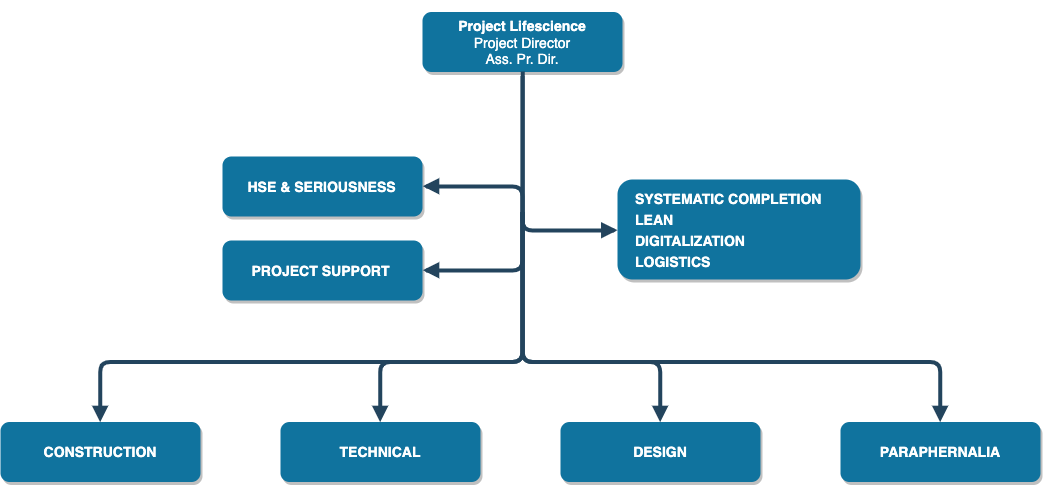
\includegraphics[width=\textwidth]{fig/lvb_diagram.png}
    \caption{Organizational structure in the Life Science Building Construction Project.}
    \label{fig:project_structure}
\end{figure}

Making sure the resulting building is a correct representation of the project vision, process management has developed a customized process. Influenced by agile processes, the method using an iterative process, starting with the vision of the building, ending up with the product; in the form of a finished building. Every iteration has the intention of getting closer to the conclusion, not concluding too early. When every discipline is taken into consideration and satisfied, the project proceeds into the next iteration. Hopefully, this makes for nothing to be redone because no crucial parts are missing. Having these iterations depends on involving disciplines and actors early in the process, which is shown to be demanding.

The implementation management divides into four levels: (1) the Milestones: A significant planned completion of a part of the project, e.g., completion of a floor or start of a new project phase; (2) Key Points: Key Points is less significant, and with a shorter time frame than milestones, but in the same way an indication of completion; (3) Deliveries: Deliveries consists of several Key Points, e.g., finishing a room or design of a floor; and (4) Actions: Actions is everything needed to be done to complete a Delivery. 

\subsubsection{Interaction, communication and cooperation}

\subsubsection{Project management software}

\begin{itemize}
    \item Cogito: Planning and getting information about how much can run in parallel and serial. 
    \item Revit and DRofus
    \item Solibri
    \item Interacso
    \item BIM
\end{itemize}
 
\subsubsection{Project management methods} 
Lean Constructing heavily influences project management in the LSB-project. Some ceremonies applied weekly are Weekly Work Plan (WWP). Every Monday, stakeholders are gathered, checking the status of the project. Identifying progress or mostly lack of it, using Cogito. Deliveries or Key Points are highlighted, and issues been raised. Keeping every stakeholder informed about the status of the project. 


\cleardoublepage